\documentclass[tikz]{standalone}
% \usepackage{amsmath}
\usetikzlibrary{arrows,decorations.markings,fit,matrix,positioning,shapes}
\tikzset{
    % >=latex,
    mymatrix/.style={matrix of nodes, nodes=typetag, row sep=.2em},
    mycontainer/.style={draw=gray, inner sep=.1ex},
    typetag/.style={draw=gray, inner sep=1ex, anchor=west},
    title/.style={draw=none, color=gray, inner sep=0pt},
    line/.style={},
    arrowfwd/.style={decoration={markings,mark=at position 1 with {\arrow[scale=2,>=stealth]{>}}},postaction={decorate}},
    arrowboth/.style={decoration={markings,mark=at position 0.15 with {\arrow[scale=2,>=stealth]{<}},mark=at position 1 with {\arrow[scale=2,>=stealth]{>}}},postaction={decorate}},
    borderthick/.style={draw,draw=black!50,thick},
    recwht/.style={draw,minimum width=3cm,minimum height=2cm,align=center,text width=3cm,text=black,fill=white,draw=black,thick},
    recdgry/.style={draw,minimum width=3cm,minimum height=2cm,align=center,text width=3cm,text=white,fill=black!50,draw=black!70,thick},
    recred/.style={draw,minimum width=3cm,minimum height=2cm,align=center,text width=3cm,text=black,fill=red!30,draw=black!50,thick},
    squorg/.style={draw,minimum width=2cm,minimum height=2cm,align=center,text width=2cm,text=orange,fill=white,draw=orange!50,thick},
    rndred/.style={rounded corners=1cm,draw,minimum width=3cm,minimum height=2cm,align=center,text width=3cm,text=red,fill=rwhite,draw=red!30,thick},
    rndyel/.style={rounded corners=1cm,draw,minimum width=3cm,minimum height=2cm,align=center,text width=3cm,text=yellow,fill=white,draw=yellow!50,thick},
    diared/.style={diamond,draw,minimum width=3cm,minimum height=2cm,align=center,text width=3cm,text=red,fill=white,draw=red!30,thick,aspect=2},
    diayel/.style={diamond,draw,minimum width=3cm,minimum height=2cm,align=center,text width=3cm,text=black!70,fill=yellow!30,draw=black!70,thick,aspect=2},
    diayel2/.style={diamond,draw,minimum width=3cm,minimum height=2cm,align=center,text width=3cm,text=black!70,fill=yellow!30,draw=black!70,thick,aspect=1.5},
    diawht/.style={diamond,draw,minimum width=3cm,minimum height=2cm,align=center,text width=3cm,text=black,fill=white,draw=black,thick,aspect=2},
    diawht2/.style={diamond,draw,minimum width=3cm,minimum height=2cm,align=center,text width=3cm,text=black,fill=white,draw=black,thick,aspect=1.5},
    elwht/.style={ellipse,draw,minimum width=3cm,minimum height=2cm,align=center,text width=2cm,text=black,fill=white,draw=black,very thick},
    cirblu/.style={circle,draw,minimum width=2cm,minimum height=2cm,align=center,text width=2cm,text=blue,fill=white,draw=blue!50,very thick},
    cirred/.style={circle,draw,minimum width=2cm,minimum height=2cm,align=center,text width=2cm,text={rgb:red,255;green,0;blue,122},fill=white,draw={rgb:red,255;green,0;blue,122},very thick},
    cirpur/.style={circle,draw,minimum width=2cm,minimum height=2cm,align=center,text width=2cm,text={rgb:red,130;green,60;blue,250},fill=white,draw={rgb:red,130;green,60;blue,250},very thick},
    cylwht/.style={cylinder,draw,shape aspect=.5,cylinder uses custom fill,cylinder end fill=white,minimum width=1cm,minimum height=1cm,cylinder body fill=white,opacity=1,scale=1,draw=black!50,thick,rotate=90},
    cyldgry/.style={cylinder,draw,shape aspect=.5,cylinder uses custom fill,cylinder end fill=white,minimum width=1cm,minimum height=1cm,cylinder body fill=black!50,opacity=1,scale=1,draw=black!70,thick,rotate=90}
}
\begin{document}
    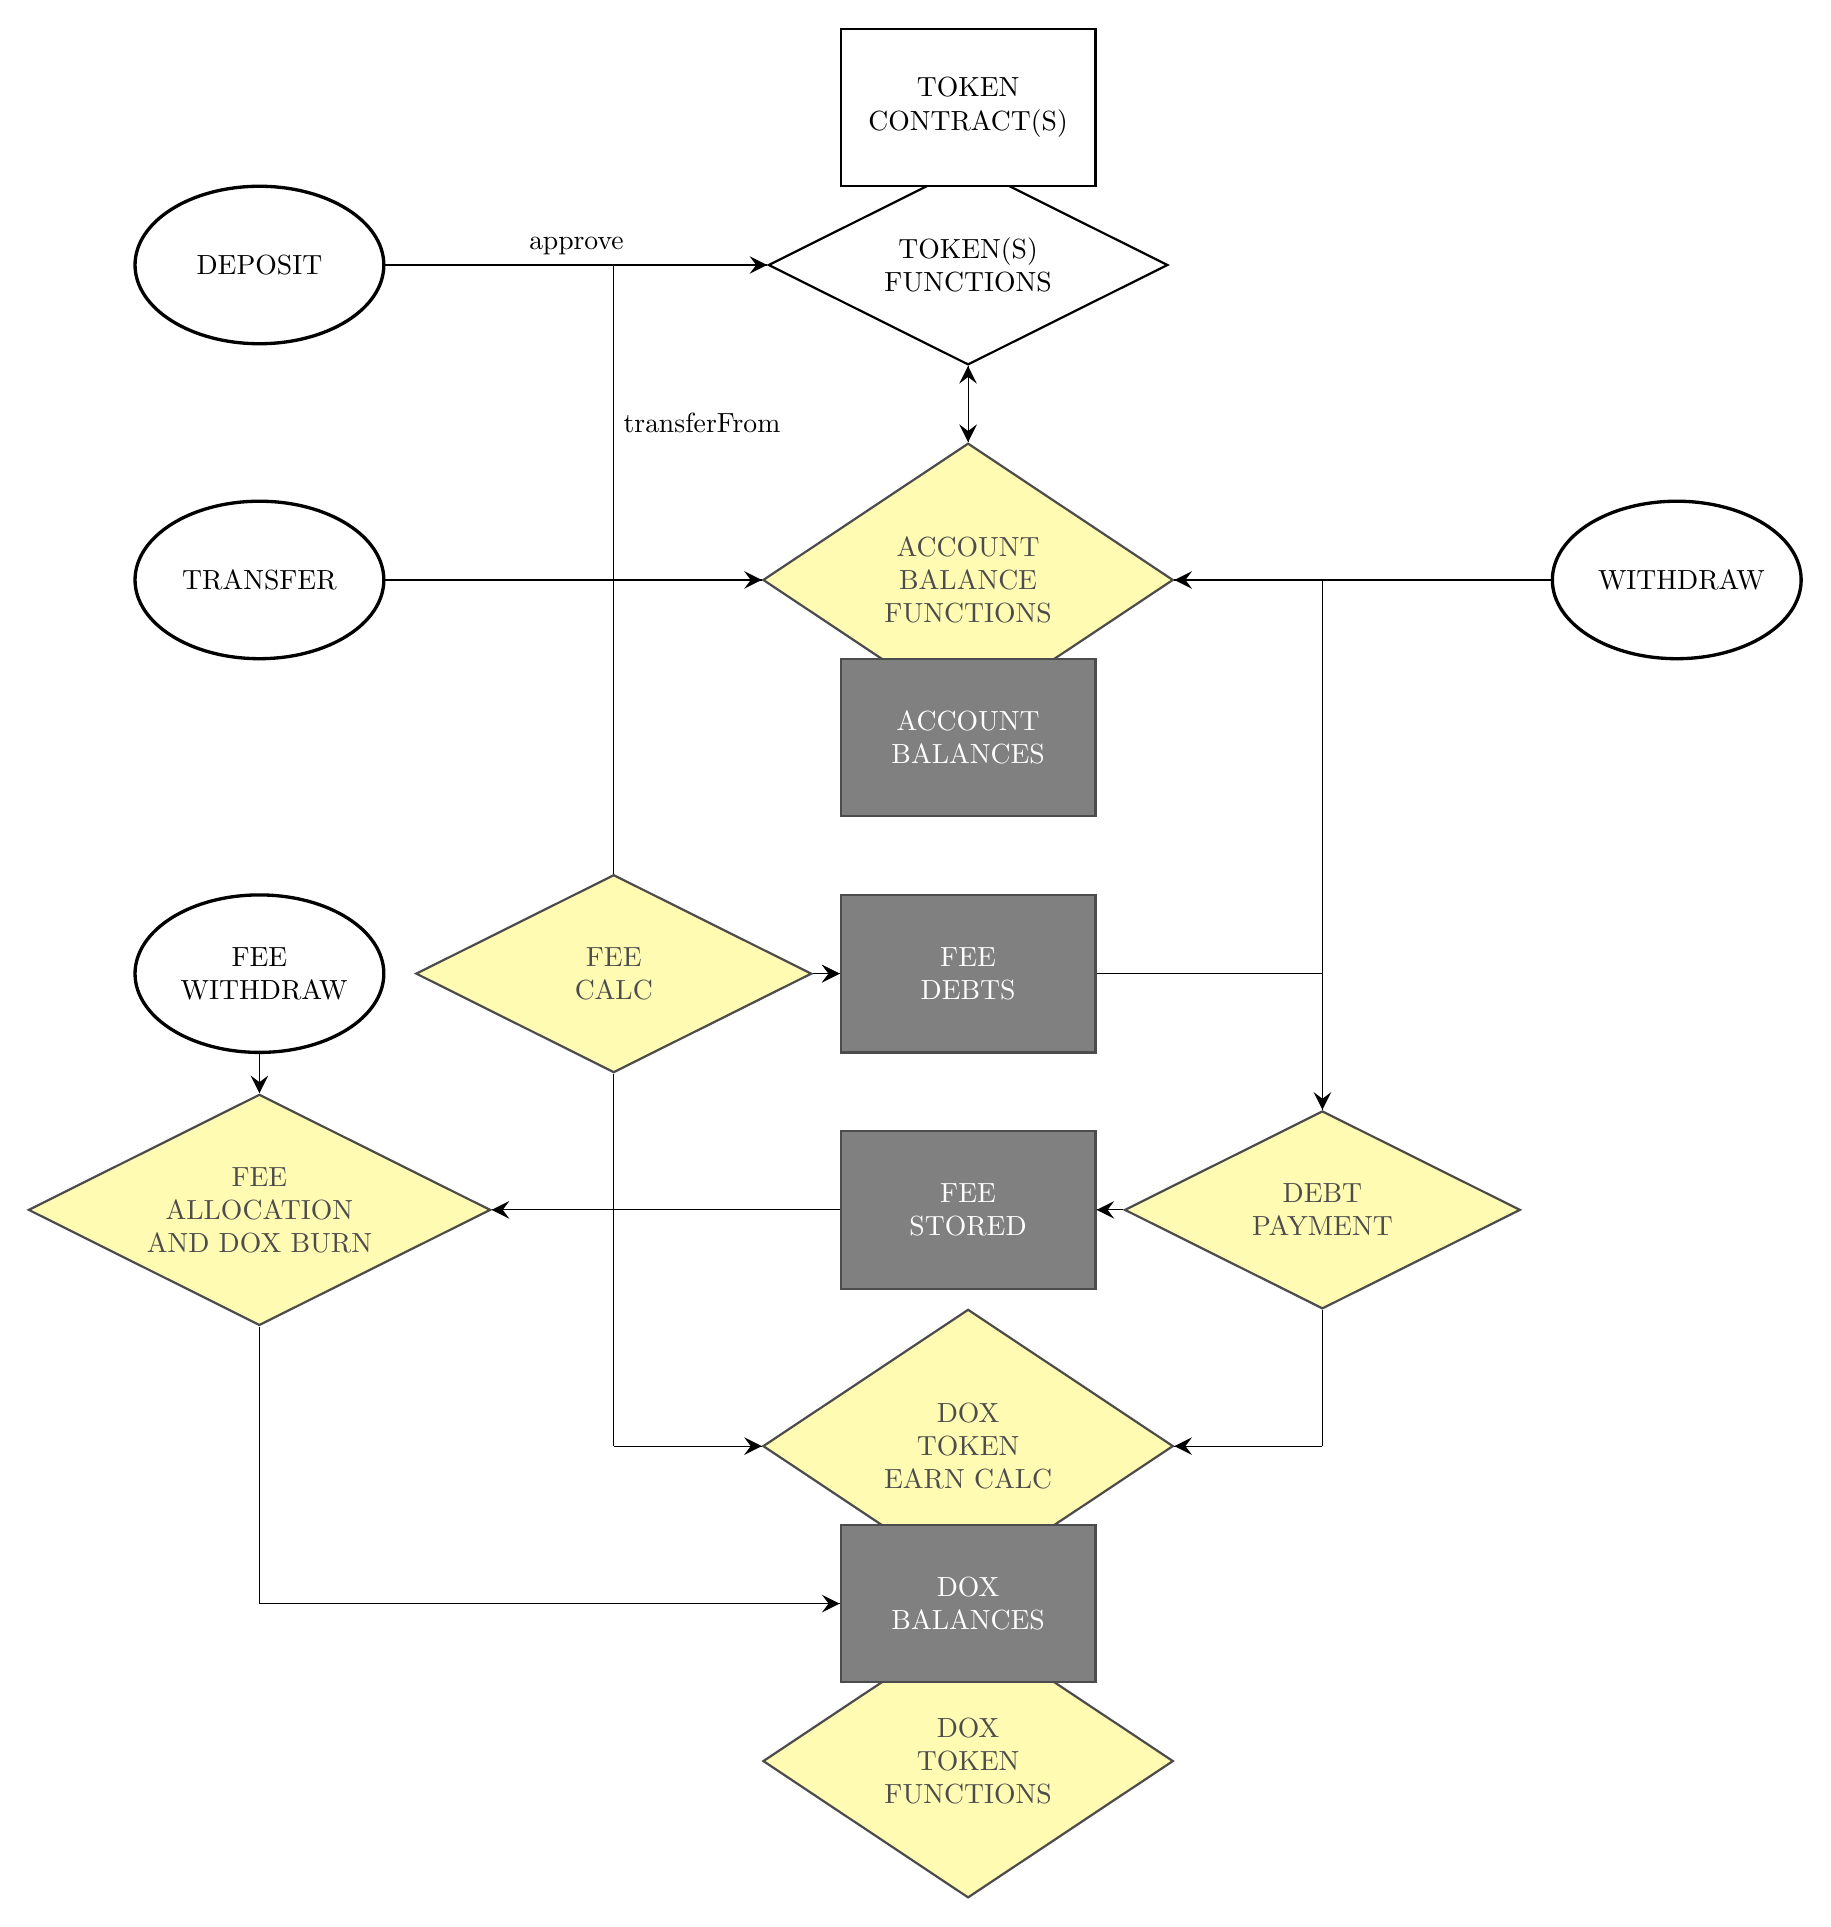
\begin{tikzpicture}[x=4.5cm,y=2cm]
        \node[elwht] (trns) at (0,1) {TRANSFER};
        \node[elwht] (dep) at (0,3) {DEPOSIT};
        \node[diawht] (tcfunc) at (2,3) {TOKEN(S) FUNCTIONS};
        \node[recwht] (tc) at (2,4) {TOKEN\\CONTRACT(S)};
        \node[diayel2] (abalfunc) at (2,1) {ACCOUNT BALANCE\\FUNCTIONS};
        \node[recdgry] (abal) at (2,0) {ACCOUNT BALANCES};
        \node[diayel] (feecalc) at (1,-1.5) {FEE\\CALC};
        \node[recdgry] (feedebt) at (2,-1.5) {FEE\\DEBTS};
        \node[recdgry] (fbal) at (2,-3) {FEE\\STORED};
        \node[diayel2] (dearn) at (2,-4.5) {DOX\\TOKEN EARN CALC};
        \node[diayel2] (dfunc) at (2,-6.5) {DOX\\TOKEN FUNCTIONS};
        \node[recdgry] (dbal) at (2,-5.5) {DOX\\BALANCES};

        \node[elwht] (wdrwl) at (4,1) {WITHDRAW};
        \node[diayel] (dpmt) at (3,-3) {DEBT\\PAYMENT};

        \node[elwht] (feewdrwl) at (0,-1.5) {FEE\\WITHDRAW};
        \node[diayel] (feealloc) at (0,-3) {FEE\\ALLOCATION\\AND DOX BURN};

        \begin{scope} %[every path/.style={-latex}]
            \draw[arrowfwd] (trns) -- (abalfunc);
            \draw[arrowfwd] (tcfunc) -- (abalfunc);
            \draw[arrowfwd] (abalfunc) -- (tcfunc);
            \draw[arrowfwd] (dep) -- (tcfunc) node[midway, above] {approve};
            \draw[line] (1,3) -- (1,1) node[midway, right] {transferFrom};
            % \draw[arrowfwd] ($(v2)!.5!(v3)$) -- ;
            % \draw[line] (1,0) -- (1,-1.2);
            % \draw[arrowfwd] (abalfunc) -- (abal);
            \draw[line] (1,1) -- (feecalc);
            \draw[arrowfwd] (feecalc) -- (feedebt);
            \draw[arrowfwd] (feecalc) -- (feedebt);
            \draw[line] (feecalc) -- (1,-4.5);
            \draw[arrowfwd] (1,-4.5) -- (dearn);
            \draw[arrowfwd] (3,1) -- (dpmt);
            \draw[line] (feedebt) -- (3,-1.5);
            \draw[arrowfwd] (dpmt) -- (fbal);
            \draw[arrowfwd] (wdrwl) -- (abalfunc);
            \draw[line] (dpmt) -- (3,-4.5);
            \draw[arrowfwd] (3,-4.5) -- (dearn);
            \draw[arrowfwd] (feewdrwl) -- (feealloc);
            \draw[arrowfwd] (fbal) -- (feealloc);
            \draw[line] (feealloc) -- (0,-5.5);
            \draw[arrowfwd] (0,-5.5) -- (dbal);
        \end{scope}
    \end{tikzpicture}
\end{document}